\documentclass[11pt]{article}
\usepackage{tikz}



\title{ Title}
\author{ Author }
\date{\today}

\begin{document}


\subsection{Notations}
$\odot$ is the Hadamart productsss

\section{Forward propagation}
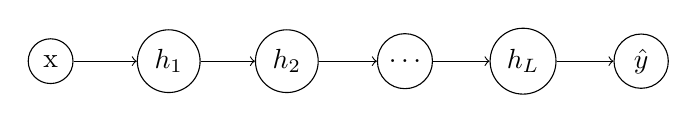
\begin{tikzpicture}[node distance = {15mm}, main/.style = {draw, circle}]
    \node[main] (x) {x};
    \node[main] (h1) [right of=x] {$h_{1}$};
    \node[main] (h2) [right of=h1] {$h_{2}$};
    \node[main] (rest) [right of=h2] {$\dots$};
    \node[main] (hl) [right of=rest] {$h_{L}$};
    \node[main] (y) [right of=hl] {$\hat{y}$};
    \draw[->] (x) -- (h1);
    \draw[->] (h1) -- (h2);
    \draw[->] (h2) -- (rest);
    \draw[->] (rest) -- (hl);
    \draw[->] (hl) -- (y);    
\end{tikzpicture}

\[a^{l} = f^{l}(o^{l})\]
\[o^{l} = W^{l}a^{l-1}+b^{l}\]
Therefore, if we omit the bias terms, we have that
\[
y=
f^L(W^L
	f^{L-1}(W^{L-1}(
		\dots
	))
)
\]



\section{Backward propagation}
\subsection{How to compute the gradient slice of $w_{i}^L$ recursively}
\[
\nabla {\frac{c}{ w^l}} 
= 
(\sum_{i} \nabla \frac{a^{l}_{i}}{ w^l} )
[\nabla \frac{c}{a^l}]^T
\odot
\overrightarrow{\frac{\partial o^L}{\partial w_{i}^L}}
=
\overrightarrow{\frac{\partial c}{\partial a^L}}
\odot
\overrightarrow{\frac{\partial a^L}{\partial o^L}}
\odot
\overrightarrow{\frac{\partial o^L}{\partial w_{i}^L}}
\]
\[
\overrightarrow{\frac{\partial c}{\partial a^L}}
=
\overrightarrow{\frac{\partial o^{L+1}}{\partial a^L}}
\sum_{i} \frac{\partial c}{\partial o^{L+1}_{i}} 
=
\overrightarrow{\sum_{j} w_{i, j}^{L+1}}
\sum_{i} \frac{\partial c}{\partial o^{L+1}_{i}}
=
\overrightarrow{\sum_{k} w_{\forall, k}^{L+1} 
\frac{\partial c}{\partial o^{L+1}_{k}}}\\
\]
\[
\overrightarrow{\frac{\partial o^L}{\partial w_{i}^L}} = a^{L-1}
\]
If we pose $\lambda = \frac{\partial c}{\partial o}$ and use the previous
results we can obtain a compact recursive formulation of the gradient
slice $w_{i}^L$
\[
\overrightarrow{\frac{\partial c}{\partial w_{i}^L}} 
= 
\lambda^{L}a^{L-1}, 
\]



\end{document}
